% !TeX spellcheck = en_GB
\documentclass[a4paper, 12pt]{scrartcl}

\setkomafont{title}{\rmfamily}
\addtokomafont{disposition}{\rmfamily}

\usepackage[english]{babel}
\usepackage[T1]{fontenc}
\usepackage{lmodern}
\usepackage[utf8]{inputenc}

\usepackage{amsmath}
\usepackage{amssymb}
\usepackage{amsfonts}
\usepackage{amsthm}
\usepackage{bbm}


\usepackage{hyperref}

%\usepackage{icomma}

\usepackage{graphicx}
\usepackage{subcaption}

\usepackage{enumitem}

\usepackage{placeins}

\usepackage[dvipsnames]{xcolor}
\usepackage{mdframed}

\definecolor{light-gray}{gray}{0.975}


\newmdenv[backgroundcolor=light-gray, linecolor=White, leftmargin=-0.25\paperwidth+0.5\linewidth, rightmargin=-0.25\paperwidth+0.5\linewidth, innerleftmargin=0.25\paperwidth-0.5\linewidth, innerrightmargin=0.25\paperwidth-0.5\linewidth]{algorithm}

% leftmargin=-10pt, rightmargin=-10pt]{algorithm}

\usepackage{tablefootnote} 
\makeatletter 
\AfterEndEnvironment{mdframed}{%
	\tfn@tablefootnoteprintout% 
	\gdef\tfn@fnt{0}% 
}

\newcommand{\bfbeta}{\boldsymbol{\beta}}
\newcommand{\bflambda}{\boldsymbol{\lambda}}
\newcommand{\bfmu}{\boldsymbol{\mu}}
\newcommand{\bfalpha}{\boldsymbol{\alpha}}
\newcommand{\bfx}{\mathbf{x}}
\newcommand{\inner}[2]{\left\langle #1, #2 \right\rangle}
\newcommand{\var}{\operatorname{\mathbb{V}ar}}
\newcommand{\ex}{\operatorname{\mathbb{E}}}
\newcommand{\cor}{\operatorname{\mathbb{C}orr}}

%opening
\title{\vspace{0.7cm}{\Large \textbf{TILM3592\\Advanced Statistical Learning}}\\{\LARGE \bfseries Learning Diary}}
\author{{\large NAME}\\
{ MATR.}}
\date{}

\begin{document}
\maketitle


\section{Linear Model Selection and Regularization, Shrinkage}

The objective is to find a good (``best'') model of the form
\begin{equation}\label{eq:fulllinearmodel}
	\mathbf{y}=\beta_0+\beta_1\bfx_1+\ldots+\beta_p\bfx_p.
\end{equation}
One possible solution would be to just use all of the predictors, this would minimize the sum of the squared residuals on the training set but would not necessarily give a model that generalizes as well as a simpler model.
This phenomenon is called overfitting, the model overfits to the training data and performs worse than a simpler model.
Overfitting is often caused by using a model that is too complex.
For example if we have a training set containing $N$ samples of $p$ predictors we could extend the number of predictors until the number of predictors $p'$ is equal to $N$, using some suitable method of extending (for example by constructing suitable polynomials of the initial predictors).
Using all $p'$ of the predictors we would then be able to perfectly fit the training set but performance on the validation set would be awful.

In order to find a model that generalizes well we instead look for a restriction of the model (\ref{eq:fulllinearmodel}) that performs well on a hold out set/test set/validation set.
The restriction can be chosen in many ways, for example we could simply choose the best subset of the predictors.

%\newpage
\subsubsection*{Best Subset Selection}
\begin{algorithm}
For $k=1,\ldots,p$ fit all the ${p \choose k}$ models with $k$ predictors.
For each $k$ choose the model $\mathcal{M}_k$ that performs the best, here the best model can be defined as lowest $R^2$ since all the models have the same number of predictors \tablefootnote{Why not use lowest cross-validation error here too? Perhaps for computational reasons or if no validation set exists.}.
In the end choose the final model by looking at some measure that take into account the complexity of the model (how many predictors were used, $k$) or just using the cross-validation error (either the one predicted using $k$-fold cross-validation or just the performance on a hold-out set).
There are a couple of regularly used measures that take into account the complexity of the model, for example the Akaike and Bayesian Information Criteria, Mallow's $C_p$ or the adjusted $R^2$-statistic.
\end{algorithm}

This method is computationally very expensive if the number of predictors $p$ is large.
This can be seen by looking at the sum of the binomial coefficients, $\sum_{k=0}^{p}{p \choose k}$ which equals $2^p$.
Thus $2^p$ models need to be fit and evaluated before we arrive at a final model.
There are other methods that also perform well (but they might not find the best model) with smaller algorithmic complexity.

\subsection{Stepwise Selection}
Instead of considering all $2^p$ of the models that the best subset selection  algorithm does the following algorithms only consider $p(p+1)/2+1$ models, drastically cutting down on the amount of needed work.
For both of the following algorithms this is done by iteratively starting with some model and modifying it.


\subsubsection*{Forward Stepwise Selection}
\begin{algorithm}
Forward stepwise selection starts with $\mathcal{M}_0$ which is the model containing only the intercept term.
The next model, $\mathcal{M}_1$, is selected by considering the $p$ models we get by including each of the $p$ predictors left separately.
The best of these models is the one with lowest $R^2$ and is denoted with $\mathcal{M}_1$.
This process of selecting one predictor to add to the model at each step is repeated until the model contains all predictors ($p$ times).
The selection fo the final model is similar to the final model selection of the best subset selection algorithm, using some criteria that takes model complexity into account.

At step $k=1,\ldots,p$ we need to fit and evaluate $p-(k-1)$ models.
The total number of models evaluated is then
\begin{equation*}
\sum_{k=1}^{p} \left(p-(k-1)\right) + 1=1+\sum_{k=1}^{p} k = p(p+1)/2+1,
\end{equation*}
where the final $+1$ term is for fitting the $\mathcal{M}_0$ model.
\end{algorithm}

%\begin{mdframed}[backgroundcolor=Goldenrod, linecolor=White]

\subsubsection*{Backwards Stepwise Selection}
\begin{algorithm}
In contrast to forwards stepwise selection backwards stepwise selection is when we start with the full model, $\mathcal{M}_p$, and remove one predictor at each step to iteratively get the models $\mathcal{M}_{p-1},\mathcal{M}_{p-2},\ldots,\mathcal{M}_0$.
The selection of a final model is again the same as for best subset selection and the analysis of complexity is the same as for forwards stepwise selection.
\end{algorithm}

An important thing to note is that stepwise selection does not necessarily give the same model as best subset selection (in other words, not always the best model).
This is because once a predictor is included/dropped we can not choose to drop/reinclude it at a later point even though that might be advantageous.

There are also other ways of doing forwards and backwards stepwise selection, for instance we can choose to use the $F$-statistic to evaluate what predictors to include/drop.

\subsection{Regularization, Shrinkage}
Another approach is to modify the loss-functions used in ordinary linear regression.
Often this is done by adding some kind of penalty to the loss-function, e.g. instead of solving
\begin{equation*}
	\operatornamewithlimits{argmin}_{\bfbeta}\left( \sum_{i=1}^{N}\left(y_i-\beta_0-\bfx_i^\intercal\bfbeta \right)^2\right)
\end{equation*}
we solve
\begin{equation*}
	\operatornamewithlimits{argmin}_{\bfbeta}\left( \sum_{i=1}^{N}\left(y_i-\beta_0-\bfx_i^\intercal\bfbeta\right)^2+\text{penalty}\right)
\end{equation*}
where the penalty often is some function of the coefficients that biases the algorithm towards a simpler model.

\subsubsection*{Ridge Regression}
\begin{algorithm}
Penalize the coefficients by choosing $\lambda\left\|\bfbeta\right\|^2$ as the penalty function.
The optimization problem to be solved is then
\begin{equation*} \hat{\bfbeta}^\mathrm{r}=\operatornamewithlimits{argmin}_{\bfbeta}\left( \sum_{i=1}^{N}\left(y_i-\beta_0-\bfx_i^\intercal\bfbeta\right)^2+\lambda\left\|\bfbeta\right\|^2_2\right),
\end{equation*}
where $\lambda$ is a positive real-valued (tuning) parameter chosen by cross-validation.
The solution is given by
\begin{equation*}
	\hat{\bfbeta}^\mathrm{r}=\left(\mathbf{X}^\intercal\mathbf{X}+\lambda\mathbf{I}\right)^{-1}\mathbf{X}^\intercal\mathbf{y}
\end{equation*}
where $\mathbf{X}$ is the $\left(N\times p\right)$ matrix containing all the observations.
\end{algorithm}

%TODO In practice SVD is useful for solving? PCs?

\subsubsection*{Lasso Regression}
\begin{algorithm}
Instead of penalizing the regular euclidean (2-) norm of the coefficient $\bfbeta$ we penalize the 1-norm of $\bfbeta$.
The optimization problem is then of the form
\begin{equation}\label{eq:lasso}
	\bfbeta^\mathrm{l}=\operatornamewithlimits{argmin}_{\bfbeta}\left(\sum_{i=1}^{N}\left(y_i-\beta_0-\bfx_i^\intercal\bfbeta\right)^2+\lambda\left\|\bfbeta\right\|_1\right)
\end{equation}
with no analytical solution.
Since no analytical solution exists many efficient methods of numerically solving the optimization problem have been developed, many based on techniques in optimization theory and convex analysis.
Here $\lambda$ is also a tuning parameter determined using cross-validation.
\end{algorithm}

Analysing the role of the $\lambda$-parameter a bit more we discover that if we try to use Lagrange multipliers to solve the following optimization problem
\begin{equation*}
	\begin{aligned}
	\operatornamewithlimits{argmin}_{\bfbeta} & & &\left(\sum_{i=1}^{N}\left(y_i-\beta_0-\bfx_i^\intercal\bfbeta\right)^2\right)\\
	\text{subject to} & & & \left\|\bfbeta\right\|_1 \leq t
	\end{aligned}
\end{equation*}
we recover the optimization problem (\ref{eq:lasso}) solved in Lasso regression (up to some constants that do not matter when solving for stationary points of the Lagrange function).
There is then a one-to-one correspondence between the parameters $\lambda$ and $t$ and solving either problem is the same as solving the other problem for some particular combination of parameters.

The interpretation is that the coefficient $\bfbeta$ is constrained to the 1-sphere (a square standing on one corner in 2 dimensions) with radius $t$.
Figure \ref{fig:lassopenalty} illustrates how this can have the effect of selecting variables by choosing $\bfbeta^\mathrm{l}$ such that some coordinates are equal to 0, meaning that some covariates are left outside of the final model.

For ridge regression the same can be done but here the result is that the coefficients are restricted to the regular (Euclidean) 2-sphere (a circle in 2 dimensions).
This does not in general have the effect of selecting variables, which can be seen in figure \ref{fig:ridgepenalty}.

\begin{figure}[h]
	\begin{subfigure}{.5\textwidth}
		\centering
		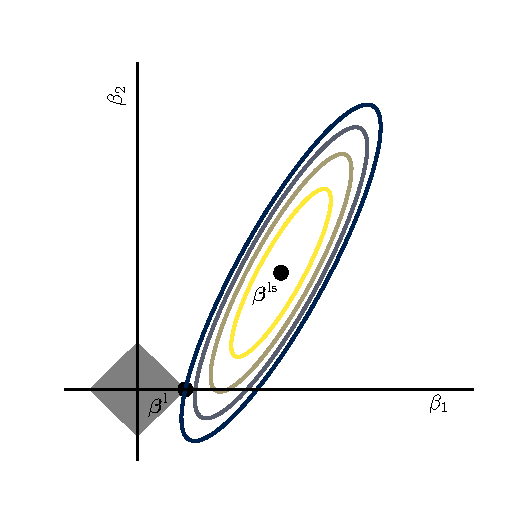
\includegraphics[width=.8\linewidth, clip, trim={10mm 10mm 10mm 10mm}]{Figure1.pdf}
		\label{fig:lassopenalty}
		\caption{Result of Lasso regression with $t=1$.}
	\end{subfigure}
	\begin{subfigure}{.5\textwidth}
		\centering
		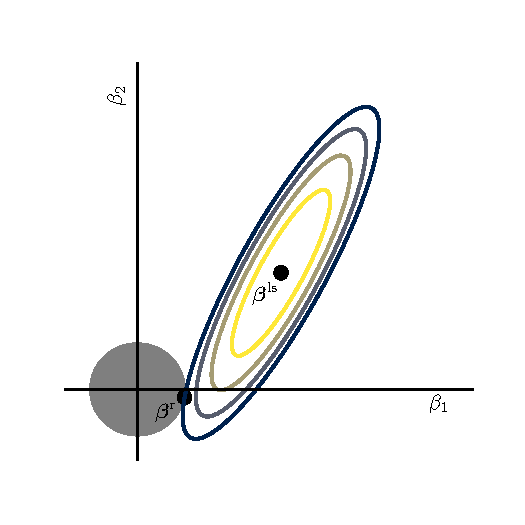
\includegraphics[width=.8\linewidth, clip, trim={10mm 10mm 10mm 10mm}]{Figure2.pdf}
		\label{fig:ridgepenalty}
		\caption{Result of ridge regression with $t=1$.}
	\end{subfigure}
	\caption{Figures illustrating the effect of the variables $t$ and $\lambda$ on the optimal values.
	The coefficient chosen by ordinary least squares is indicated by $\bfbeta^\mathrm{ls}$ with Lasso and ridge regression coefficients indicated by $\bfbeta^\mathrm{l}$ and $\bfbeta^\mathrm{r}$.
	The contours are the error (lines) and penalty (grey) parts of the loss function.}
\label{fig:fig}
\end{figure}


\subsection{Linear models utilising dimensionality reduction}
First we acquaint ourselves with a common method for dimensionality reduction.
The idea when doing dimensionality reduction is to represent the data in a less complex way without losing too much information.
For example we can try to represent the data in a new coordinate system with a smaller dimension than before while keeping as much of the variance in the model as possible.

\subsubsection*{Principal Components Analysis}
Principal components analysis is when the idea above is implemented so that we first try to find a vector $\mathbf{v}_1$ to project the new data on such that the variance of the projection is maximized.
The variance of a random variable is defined as $\var\left(\bfx\right):=\ex\left[\left(\bfx-\bfmu\right)^\intercal\left(\bfx-\bfmu\right)\right]=\ex\left(\inner{\bfx-\bfmu}{\bfx-\bfmu}\right)$ and if the random variable is centred so that the mean is equal to $\mathbf{0}$ this is equal to just $\ex\left(\bfx^\intercal\bfx\right)=\ex\left(\inner{\bfx}{\bfx}\right)$.
The projection of a random variable $\bfx$ on a vector $\mathbf{v}$ is equal to $\frac{\inner{\bfx}{\mathbf{v}}\mathbf{v}}{\left\|\mathbf{v}\right\|^2}$ where the scalar $\frac{\inner{\bfx}{\mathbf{v}}}{\left\|\mathbf{v}\right\|}$ says how far along the unit vector $\frac{\mathbf{v}}{\left\|\mathbf{v}\right\|}$ we should travel so that the random variable $\bfx$ is as close as possible.
Since all the projections will be lying on the vector $\mathbf{v}$ it is enough to take the difference between the scalars $\frac{\inner{\bfx}{\mathbf{v}}}{\left\|\mathbf{v}\right\|}$ when calculating the variance.
The variance of the projection is then equal to:
\begin{equation*}
	\var\left(\frac{\inner{\bfx}{\mathbf{v}}}{\left\|\mathbf{v}\right\|}\right)=\ex\left[\left(\frac{\inner{\bfx}{\mathbf{v}}}{\left\|\mathbf{v}\right\|}\right)^\intercal\left(\frac{\inner{\bfx}{\mathbf{v}}}{\left\|\mathbf{v}\right\|}\right)\right]=\ex\left[\frac{\left(\bfx^\intercal\mathbf{v}\right)^\intercal\left(\bfx^\intercal\mathbf{v}\right)}{\left\|\mathbf{v}\right\|^2}\right]=\ex\left[\frac{\mathbf{v}^\intercal\bfx\bfx^\intercal\mathbf{v}}{\mathbf{v}^\intercal\mathbf{v}}\right].
\end{equation*}
Using $N$ samples $\bfx_1,\dots,\bfx_N$ this can be estimated by summing over the result of the previous calculation for each sample and dividing by the number of samples but since the number of samples is fixed we can ignore this step.
This can also be expressed in matrix notation by stacking the samples $\bfx_i$ as rows in $\mathbf{X}$.
The sum is then represented by the quantity
\begin{equation*}
	\frac{\mathbf{v}^\intercal\mathbf{X}^\intercal\mathbf{X}\mathbf{v}}{\mathbf{v}^\intercal\mathbf{v}}.
\end{equation*}

Finding a vector $\mathbf{v}$ that maximizes the variance of a random variable $\bfx$ projected upon it is then equal to solving the following optimization problem:
\begin{equation*}
\begin{aligned}
	\operatornamewithlimits{argmax}_{\mathbf{v}_1} & & &\frac{\mathbf{v}_1^\intercal\mathbf{X}^\intercal\mathbf{X}\mathbf{v}_1}{\mathbf{v}_1^\intercal\mathbf{v}_1}.
\end{aligned}
\end{equation*}
Scaling the vector $\mathbf{v}$ does not change the value of the objective function here so we can add the constraint $\left\|\mathbf{v}\right\|=1$ to get a unique solution. The optimization problem is then
\begin{equation*}
\begin{aligned}
\operatornamewithlimits{argmax}_{\mathbf{v}_1} & & &\mathbf{v}_1^\intercal\mathbf{X}^\intercal\mathbf{X}\mathbf{v}_1\\
\text{subject to} & & &\left\|\mathbf{v}\right\|=1
\end{aligned}
\end{equation*}
with the Lagrange function
	$\mathcal{L}\left(\mathbf{v}_1, \lambda_1\right)=\mathbf{v}_1^\intercal\mathbf{X}^\intercal\mathbf{X}\mathbf{v}_1-\lambda_1\left(\mathbf{v}_1^\intercal\mathbf{v}_1-1\right)$.
Stationary points are found by solving for points where the derivative $\frac{\mathrm{d}\mathcal{L}}{\mathrm{d}\mathbf{v}_1}=2\mathbf{v}_1^\intercal\mathbf{X}^\intercal\mathbf{X}-2\lambda_1\mathbf{v}_1^\intercal$ equals 0.
This is obviously an eigenvalue problem and the solution is given by the largest eigenvalue $\lambda_1$ of the matrix $\mathbf{X}^\intercal\mathbf{X}$  with the corresponding eigenvector $\mathbf{v}_1$.

The first \emph{principal component} of an observation $\bfx_i$ is what the projection $\inner{\bfx_i}{\mathbf{v}_1}\mathbf{v}_1$ is called.
In order to find more principal components the data can be altered by subtracting the projections of the samples on the eigenvectors and then extracting a new eigenvector in a similar way.
It turns out that first eigenvector of the new (squared) data matrix will be the second eigenvector of the original and this is starting to look a lot like some sort of eigenvector decomposition of the matrix $\mathbf{X}^\intercal\mathbf{X}$ or $\mathbf{X}$, which is the approach investigated below. 

The other approach is to model the observations as the rank-$q$ linear model $f(\bflambda)=\bfmu + \mathbf{V}_q\bflambda$ where $\bflambda$ are coordinates in a $q$-dimensional space, $\bfmu$ is the location of the $p$-dimensional mean and $\mathbf{V}_q$ is a $\left(q\times p\right)$-dimensional matrix with $q$ orthonormal vectors as columns.
This is an affine hyperplane of rank $q$.
\begin{algorithm}
	We try to minimize the \emph{reconstruction error}:
	\begin{equation*}
	\begin{aligned}
		\operatornamewithlimits{argmin}_{\bfmu, \bflambda_i, \mathbf{V}_q} & & &\sum_{i=1}^{N}\left\|\bfx_i-\bfmu-\mathbf{V}_q\bflambda_i\right\|^2.
	\end{aligned}
	\end{equation*}
	By partially optimizing for $\boldsymbol{\mu}$ and $\bflambda_i$ we get $\hat{\boldsymbol{\mu}} = \bar{\bfx}$ and $\hat{\bflambda}_i=\mathbf{V}_q^\intercal \left(\bfx_i-\bar{\bfx}\right)$.
	Assuming the data is centred ($\bar{\bfx}=\mathbf{0}$) we are left with determining $\mathbf{V}_q$:
	\begin{equation*}
	\begin{aligned}
	\operatornamewithlimits{argmin}_{\mathbf{V}_q} & & &\sum_{i=1}^{N}\left\|\bfx_i-\mathbf{V}_q\mathbf{V}_q^\intercal\bfx_i\right\|^2.
	\end{aligned}
	\end{equation*}
	The solution can be constructed using the singular value decomposition $\mathbf{U}\mathbf{D}\mathbf{V}^\intercal$ of the data $\mathbf{X}$.
	Here $\mathbf{U}$ is a $\left(N\times p\right)$ orthogonal matrix, $\mathbf{D}$ is a $\left(p\times p\right)$ diagonal matrix with the eigenvalues of $\mathbf{X}$ on the diagonal ordered by size and $\mathbf{V}^\intercal$ is a $\left(p\times p\right)$ orthogonal matrix. The solution $\mathbf{V}_q$ for a given $q\leq p$ is given by the first $q$ columns of $\mathbf{V}$.
	Similarly the new reduced space is given by the first $q$ columns of $\mathbf{U}\mathbf{D}$.
	
	The interpretation is that we have projected the original space down on the first $q$ \emph{principal components} of the data.
	We also have a way to reconstruct the original data using the matrix $\mathbf{V}_q$.
\end{algorithm}

Principal components analysis also has a couple of other interpretations and properties.
For example the eigenvalues can be interpreted as the variance explained by a particular principal component.
The total variance is then given by the sum of all the eigenvalues and the ratio of variance explained to total variance is the ratio of the sum of the $q$ largest eigenvalues to the sum of all the eigenvalues.
Normally the decomposition is constructed for all $p$ principal components and a plot of the ratio of variance explained to total variance for each $q$ is used to determine when to stop.
Usually there is a sharp drop of in additional explaining power after a couple of principal components, at that point it is no longer efficient (in the interest of interpretability) to include more dimensions.

\subsubsection*{Principal Components Regression}
Now that we have a method for reducing the dimensionality of our data we could try ordinary linear regression on the new dimensions.
\begin{algorithm}
	Principal components regression is when ordinary linear regression is ran on the first $k$ principal components calculated using PCA.
	The principal components $\mathbf{z}_i$ are given by $\mathbf{z}_i=\mathbf{X}\mathbf{v}_i$ where $\mathbf{v}_i$ are the eigenvectors identified by PCA.
	Stacking the principal components columnwise in an $\left(N\times k\right)$ matrix $\mathbf{Z}$ means that the ordinary least squares solution $\bfalpha^\mathrm{ls}$ to the optimization problem
	\begin{equation*}
	\begin{aligned}
	\operatornamewithlimits{argmin}_{\bfalpha} & & &\left\|\mathbf{y}-\mathbf{Z}\bfalpha\right\|^2.
	\end{aligned}
	\end{equation*}
	is given by $\bfalpha^\mathrm{ls}=\left(\mathbf{Z}^\intercal\mathbf{Z}\right)^{-1}\mathbf{Z}^\intercal\mathbf{y}$, here everything is assumed to be centred (also $\mathbf{y}$).
\end{algorithm}


Having used the singular value decomposition a bit we can try to investigate the previous algorithms we have introduced, mainly by comparing ordinary least squares and ridge regression.
For least squares the fitted values are:
\begin{align*}
	\mathbf{X}\bfbeta^\mathrm{ls}&=\mathbf{X}\left(\mathbf{X}^\intercal\mathbf{X}\right)^{-1}\mathbf{X}^\intercal\mathbf{y}
	=\mathbf{U}\mathbf{D}\mathbf{V}^\intercal\left(\mathbf{V}\mathbf{D}^\intercal\mathbf{U}^\intercal\mathbf{U}\mathbf{D}\mathbf{V}^\intercal\right)^{-1}\mathbf{V}\mathbf{D}^\intercal\mathbf{U}^\intercal\mathbf{y}\\
	&=\mathbf{U}\mathbf{D}\mathbf{V}^\intercal\left(\mathbf{V}^\intercal\right)^{-1}\mathbf{D}^{-2}\mathbf{V}^{-1}\mathbf{V}\mathbf{D}\mathbf{U}^\intercal\mathbf{y}
	=\mathbf{U}\mathbf{U}^\intercal\mathbf{y},
\end{align*}
while for ridge regression we get:
\begin{align*}
	\mathbf{X}\bfbeta^\mathrm{r}&=\mathbf{X}\left(\mathbf{X}^\intercal\mathbf{X}+\lambda\mathbf{I}\right)^{-1}\mathbf{X}^\intercal\mathbf{y}
	=\mathbf{U}\mathbf{D}\mathbf{V}^\intercal\left(\mathbf{V}\mathbf{D}^\intercal\mathbf{U}^\intercal\mathbf{U}\mathbf{D}\mathbf{V}^\intercal+\lambda\mathbf{I}\right)^{-1}\mathbf{V}\mathbf{D}^\intercal\mathbf{U}^\intercal\mathbf{y}\\
	&=\mathbf{U}\mathbf{D}\mathbf{V}^\intercal\left(\mathbf{V}\mathbf{D}\mathbf{D}\mathbf{V}^\intercal+\lambda\mathbf{I}\right)^{-1}\mathbf{V}\mathbf{D}^\intercal\mathbf{U}^\intercal\mathbf{y}
	=\mathbf{U}\mathbf{D}\mathbf{V}^\intercal\left(\mathbf{V}\mathbf{D}\mathbf{D}\mathbf{V}^\intercal+\lambda\mathbf{V}\mathbf{V}^\intercal\right)^{-1}\mathbf{V}\mathbf{D}^\intercal\mathbf{U}^\intercal\mathbf{y}\\
	&=\mathbf{U}\mathbf{D}\mathbf{V}^\intercal\left(\mathbf{V}\left(\mathbf{D}\mathbf{D}+\lambda\mathbf{I}\right)\mathbf{V}^\intercal\right)^{-1}\mathbf{V}\mathbf{D}^\intercal\mathbf{U}^\intercal\mathbf{y}
	=\mathbf{U}\mathbf{D}\left(\mathbf{D}^2+\lambda\mathbf{I}\right)^{-1}\mathbf{D}\mathbf{U}^\intercal\mathbf{y}\\
	&=\sum_{i=1}^{p}\mathbf{u}_i\frac{d^2_i}{d^2_i+\lambda}\mathbf{u}_i^\intercal\mathbf{y}
\end{align*}
where $\mathbf{u}_i$ are the columns of $\mathbf{U}$ and $d_i^2$ are the squared singular values present in the diagonal matrix $\mathbf{D}^2$.
Using the understanding gained from the principal components analysis derivations the interpretation is that ridge regression puts more emphasis on the directions of the principal components with large singular values or in other words, the directions containing more variance are seen as more important.

This can be compared to principal components regression where directions with variance smaller than some threshold are completely ignored.
The conclusion is then that depending on how the singular values decrease (sharp drop off after some point or gradual decrease) ridge regression and principal components regression can give very similar results.

\subsubsection*{Partial Least Squares}
A drawback with principal components analysis as a tool for dimensionality reduction is that the resulting principal directions are not necessarily ``useful''.
Clearly we could use them to regularize out regression in some sense by cutting out some of the variance but if we have some response variable $\mathbf{y}$ it would make sense to also use that for the dimensionality reduction step.
This is the problem partial least squares tries to solve.

\begin{algorithm}
	Let $\mathbf{x}_i$ be the $N$-dimensional vector representing all standardized observations of the $p$th input variable.
	Then set $\mathbf{z}_1=\sum_{i=1}^{p}\inner{\mathbf{x}_i}{\mathbf{y}}\mathbf{x}_i$.
	In other words, project $\mathbf{y}$ on $\mathbf{x}_i$ for all the variables and sum this, this is our new variable to regress on.
	Now set $\boldsymbol{\theta}_1=\frac{\inner{\mathbf{z}_1}{\mathbf{y}}}{\inner{\mathbf{z}_1}{\mathbf{z}_1}}$, in other words calculate some regression.
	The fitted variables are now $\mathbf{y}_1=\boldsymbol{\theta}_1\mathbf{z}_1$.
	Now orthogonalize each input $\mathbf{x}_i$ with respect to $\mathbf{z}_1$ using the following operation:
	\begin{equation*}
		\mathbf{x}_i=\mathbf{x}_i-\frac{\inner{\mathbf{z}_1}{\mathbf{x}_i}}{\inner{\mathbf{z}_1}{\mathbf{z}_1}}\mathbf{z}_1
	\end{equation*}
	and repeat from the beginning, the only difference now is that we need to add the previous fitted variables to $\boldsymbol{\theta}_2\mathbf{z}_2$.
	
	This procedure can be repeated at most $p$ times, at which point our fitted values are equal to $\sum_{i=1}^{p}\boldsymbol{\theta}_i\mathbf{z}_i$ where the relationship between the coefficients $\boldsymbol{\theta}_i$ and input variables $\mathbf{z}_i$ is such that this is equal to ordinary least squares regression on the original input variables $\mathbf{x}_i$.
	Since the new variables $\mathbf{z}_i$ are linear combinations of the original input variables we can recover a solution $\bfbeta^\mathrm{pls}$ for the original variables even if we leave out some of the last variables.
\end{algorithm}

In conclusion, partial least squares and principal components regression are both procedures where we reshape the input space using some linear combinations.
Both of them are able to retain all the ``information'' or variance if we want to but usually they are cut of at some point.

The difference is that while the $m$th principal component $\mathbf{v}_m$ can be shown to solve the optimization problem
\begin{equation*}
	\begin{aligned}
	\operatornamewithlimits{max}_{\left\|\bfalpha\right\|=1} & & &\var\left(\mathbf{X}\bfalpha\right)\\
	\text{subject to} & & & \mathbf{v}_l^\intercal\mathbf{S}\bfalpha\text{ for }l=1,\dots,m-1,
	\end{aligned}
\end{equation*}
the partial least squares directions can be shown to solve the optimization problem
\begin{equation*}
	\begin{aligned}
	\operatornamewithlimits{max}_{\left\|\bfalpha\right\|=1} & & &\cor\left(\mathbf{y},\mathbf{X}\bfalpha\right)^2\var\left(\mathbf{X}\bfalpha\right)\\
	\text{subject to} & & & \mathbf{v}_l^\intercal\mathbf{S}\bfalpha\text{ for }l=1,\dots,m-1.
\end{aligned}
\end{equation*}
In both cases the condition $\mathbf{v}_l^\intercal\mathbf{S}\bfalpha\text{ for }l=1,\dots,m-1$, where $\mathbf{S}$ is the sample covariance matrix, ensures that the solution is uncorrelated to the previous solutions.
Apparently, the variance usually tends to dominate so the solutions from partial least squares are usually similar to the solutions of principal components regression, which is again somewhat similar to ridge regression.

\section{Tree based methods}
With tree based methods the idea is to partition the input space into smaller sections where a relatively simple model can be fit, for example just fitting the intercept of linear regression.
In this way one can approximate more complex functions.
The problem then is that we can easily start overfitting, if no two points occupy the same space one can always draw rectangles such that each rectangle is only occupied by one point but this would probably not lead to a particularly good solution.

Thus the question is more one of how we should split the input space or rather when and where.
Usually we use rectangles with sides orthogonal to the input variables to split and decide on what and where to split using some loss function.
Furthermore we always split each rectangle in each step if it is possible (a rectangle containing only one training sample can't be split).

Usually the trees are grown large (by splitting many times) until some criterion is met, for example until the node size/rectangle size is at most 5, and then splits are removed using a procedure called cost-complexity pruning.
The cost-complexity is usually a function that weighs the importance of prediction power and complexity of the tree using some hyperparameter that is usually chosen using cross-validation.

The tree $\mathcal{T}$ is pruned to find the trees $\mathcal{T}_\alpha$ that minimizes the cost-complexity $C_\alpha\left(\mathcal{T}\right)$, from these optimal trees one is chosen using cross-validation or equivalently the hyperparameter $\alpha$ is chosen.
In order to find the optimal $\mathcal{T}_\alpha$ we produce a sequence of trees using \emph{weakest-link pruning}; we remove one split at a time and we always remove the split that gives the smallest per node increase in the cost- or loss-part of the cost-complexity function.
This is repeated until no splits are left and this sequence can be shown to always contain $\mathcal{T}_\alpha = \operatornamewithlimits{argmin}_\mathcal{T}C_\alpha(\mathcal{T})$.

\subsubsection*{Regression trees}
\begin{algorithm}
For regression trees we split each rectangle so that the resulting squared residuals in the two new rectangles is minimized.
Mathematically this is expressed like this:
	\begin{equation*}
	\operatornamewithlimits{min}_{j,s}\left(\operatornamewithlimits{min}_{c_1}\sum_{\mathbf{x}_i\in \mathcal{R}_1\left(j,s\right)}\left(y_i-c_1\right)^2+\operatornamewithlimits{min}_{c_1}\sum_{\mathbf{x}_i\in \mathcal{R}_2\left(j,s\right)}\left(y_i-c_2\right)^2\right)
	\end{equation*}
	where $j$ is the splitting variable chosen among $1,\dots,p$ and $s$ is the splitting point.
The resulting rectangles are denoted by $\mathcal{R}_1\left(j,s\right)$ and $\mathcal{R}_2\left(j,s\right)$ and the inner optimization problems can be solved by setting
\begin{equation*}
c_k := \sum_{\mathbf{x}_i\in \mathcal{R}_k\left(j,s\right)}\frac{y_i}{|\{\mathbf{x}_i\in \mathcal{R}_k\left(j,s\right)\}|}
\end{equation*}
where $|\{\mathbf{x}_i\in \mathcal{R}_k\left(j,s\right)\}|=:N_k$ is the number of points in a rectangle $\mathcal{R}_k$. 
The cost or loss of a node $k$ or rectangle $\mathcal{R}_k$ in a given tree $\mathcal{T}$ is given by 
\begin{equation*}
	Q_k\left(\mathcal{T}\right):=\frac{1}{N_k}\sum_{\mathbf{x}_i\in \mathcal{R}_k}\left(y_i-c_k\right)^2
\end{equation*}
while the cost-complexity function is given by
\begin{equation*}
	C_\alpha\left(\mathcal{T}\right):=\sum_{k=1}^{|\mathcal{T}|}N_kQ_k\left(\mathcal{T}\right)+\alpha|\mathcal{T}|
\end{equation*}
where $\sum_{k=1}^{|\mathcal{T}|}N_kQ_k\left(\mathcal{T}\right)$ is the per-node complexity part of the weakest-link pruning procedure.
\end{algorithm}

\subsubsection*{Classification trees}

\begin{algorithm}
	For classification we need to change the costs $Q_k\left(\mathcal{T}\right)$ and the predictions $c_k$.
	We set
	\begin{equation*}
		c_k:=\operatornamewithlimits{argmax}_j \sum_{\mathbf{x}_i\in \mathcal{R}_k}\mathbbm{1}_{\{\text{class of }\mathbf{x}_i\text{ equals }j \}}
	\end{equation*}
	and for the cost we have some choices, either we use the misclassification error rate
	\begin{equation*}
		Q_k\left(\mathcal{T}\right)=\frac{1}{N_k}\sum_{\mathbf{x}_i\in \mathcal{R}_k}\mathbbm{1}_{\{\text{class of }\mathbf{x}_i\text{ does not equal }c_k \}}=1-p_{kc_k},
	\end{equation*}
	where $p_{kc_k}$ is the proportion of class $c_k$ in node $k$, or we can use the Gini index
	\begin{equation*}
		Q_k\left(\mathcal{T}\right)=\sum_{j\neq j'}p_{kj}p_{kj'}=\sum_{j=1}^{J}p_{kj}\left(1-p_{kj}\right)
	\end{equation*}
	or the cross-entropy/deviance
	\begin{equation*}
		Q_k\left(\mathcal{T}\right)=-\sum_{j=1}^{J}p_{kj}\ln\left(p_{kj}\right).
	\end{equation*}
	The recommendation is to grow the tree using the Gini index or the cross-entropy while pruning should be done using the misclassification error rate.
	Growing is done by solving the optimization problem
	\begin{equation*}
	\operatornamewithlimits{min}_{j,s} Q_{\mathcal{R}_1\left(j,s\right)}(\mathcal{T}) + Q_{\mathcal{R}_2\left(j,s\right)}(\mathcal{T})
	\end{equation*}
	and weakest-link pruning is the same as for the regression tree.
\end{algorithm}
The Gini index can be interpreted as some variance but we will not consider that now.

A decision tree is a useful model for since they can be thought of as approximating human decision making.
This means that they focus on the most important variables first, since they improve the predictions the most.
This means that we can use a decision tree to get some measure of how important a variable is.

\subsection{Bagging, Boosting and Random Forests}
\subsubsection*{Bagging}
Decision trees have high variance in the sense that if we split the data into two datasets we will most likely get different predictions.
\emph{bootstrap aggregation} or \emph{bagging} is a way to reduce the variance of statistical learning methods.
The idea is that the variance of the estimate of the mean $\bar{\mathbf{z}}$ decreases if we take multiple samples so by averaging many estimates we get a better estimate with less variance without overfitting.
Of course this procedure can be used for many statistical learning methods but we will focus on trees.

\begin{algorithm}
	For decision trees we fit many relatively deep trees to different datasets that are sampled using the bootstrap.
	The predictions will be the average of the outputs for regression problems and the majority vote of the outputs for classification problems.
	Since the trees are deep they will have low bias but high variance but this is not a problem since we average over many estimates so the variance of the average of the outputs is decreased.
	
	This procedure also comes with the additional benefit of giving us an estimate for the test-set error using the \emph{out-of-bag errors}.
	We can take an observation and leave out all the trees fit on that observation when predicting.
	If the number of bags is sufficiently large, this will end up approximating the leave-one-out cross-validation error.
\end{algorithm}

Unfortunately since we get many trees we lose some interpretability.
The largest con is that we can not get the same variable importance interpretation.
Fortunately we can approximate the importance of a variable using the residual sum of squares measure or the Gini index.
We get an estimate of variable importance by averaging (over all trees) the sum of the decreases in variance gained by splitting on a variable (in each tree).

\subsubsection*{Boosting (AdaBoost)}
Here the idea is to produce a sequence of weak classifiers and take the weighted majority vote of their outputs.
Here a weak classifier means a classifier that only performs a bit better than random guessing.
The sequence of classifiers is made so that they try to cover each others weaknesses, this is accomplished using weighted sampling.
Like bagging this procedure can be applied to many different statistical learning methods to improve the results but we will focus on decision trees.

\begin{algorithm}
	We begin by fitting a shallow tree to a dataset sampled using an unweighted bootstrap, call the resulting decision tree $G_1(\bfx)$.
	The second decision tree $G_2(\bfx)$ we fit to a dataset sampled using a weighted bootstrap.
	The weights are chosen so that we give observations that are misclassified or have a large residual a higher weight while correctly classified observations get a lower weight.
	This is continued for a number of steps and the estimator only gets stronger since each successive tree tries to focus on areas that previous trees find problematic.
	The final output is either a weighted average or a weighted majority vote.
	The weights can be determined using relative performance on the whole dataset.
\end{algorithm}

Since we again have many different trees we lose a bit of interpretability but we can still get the same estimate of variable importance as we get in the bagging case.

\subsubsection*{Random Forest}
As the name implies, the random forest algorithm is a model with many trees where we have incorporated some sense of randomness.
The idea here is that we use the bagging approach but we don't always split on the optimal variable.

\begin{algorithm}
	Proceed as usually with the bagging method but always randomly select $m\leq p$ variables as candidates for splitting, typically we choose $m=\sqrt{p}$ or $m=1$ candidates for splitting.
\end{algorithm}

This decorrelates our data in some sense which is helpful since for correlated random variables we can't decrease the variance just by adding more bags.
This can be seen by looking at the variance of the average of the identically distributed random variables $B$:
\begin{equation*}
	\var\left(\bar{B}\right)=\rho\sigma^2+\frac{1-\rho}{B}\sigma^2
\end{equation*}
where the first part is zero if the variables are uncorrelated but for correlated variables we can't go below $\rho\sigma^2$.
Thus it is helpful to reduce the correlation between the estimators, that is, we force the trees to look different by restricting what they can split on.

Again, we can get an estimate of the importance of a variable in the same way as with bagging.

\section{Clustering}
There are two principal ideas that govern how clustering algorithms work, either we choose hierarchical way to cluster where each cluster can be split into smaller clusters or merged into larger clusters in a hierarchical way, then we choose how many clusters to use or we can guess how many clusters to use and try to cluster the data into that many clusters in an unhierarchical way.
Both methods are examples of unsupervised learning since we do no need any output variables to cluster, this is similar to principal components analysis.

\subsubsection*{$K$-means}
$K$-means clustering is a simple example of an unhierarchical algorithm, we have a predetermined number of clusters $K$ that we assign the observations to based on closeness.
The clusters are represented by centroids and we determine the location of the centroids in the following way:
\begin{algorithm}
	First assign the observations randomly to clusters and calculate the centres of the clusters.
	Now reassign all the observations to the closest centre and recalculate the centres, this is repeated until the centres don't change any more.
	
	We select the number of clusters $K$ by minimizing the within cluster variance.
	This procedure gives a local optimum for
	\begin{equation*}
		\operatornamewithlimits{min}_{C_1,C_2,\dots,C_K}\sum_{k=1}^{K}\frac{1}{|C_k|}\sum_{i, i'\in C_k}\sum_{j=1}^{p}(x_{ij}-x_{i'j})^2.
	\end{equation*}
\end{algorithm}

Since it is only a local optimum the initial assignment matters and we need to try many times.

\subsection{Hierarchical clustering}
We build trees of clusters either from the top or from the bottom.

\subsubsection*{Bottom-up}
\begin{algorithm}
We start with all observations in their own cluster, at each step we merge the two clusters that are closest to each other.
Closeness can be measured in many different ways, more about this later.
\end{algorithm}

\subsubsection*{Top-down}
\begin{algorithm}
We start with all observations in one cluster and split this cluster so that the greatest between group distance is achieved.
Distance between clusters can again be measured in different ways
\end{algorithm}

\subsubsection*{Linkage}
Linkage is what we call our way of measuring distances between things, so called dissimilarity measures.
There are a couple of commonly used ones:
\begin{itemize}
	\item Single Linkage: The distance between two clusters is defined as the smallest euclidean distance between the two clusters.
	\item Group Average: The distance between two clusters is defined as the distance between the cluster averages.
	\item Complete Linkage: The distance between two clusters is defined as the largest euclidean distance between the two clusters.
\end{itemize}
All the linkages will usually perform differently, Complete Linkage will try to keep the clusters as compact as possible while Single Linkage can produce chains that can be long but thin, giving a less compact cluster.
The Group Average is something of a compromise between the two.

The number of clusters is usually selected using a drawing of the resulting tree where the vertical lengths represent the drops in dissimilarity of a split.
Such a tree is called a dendrogram and, like with principal components analysis, usually there are natural points that seem logical to split at.

\section{Support Vector Machines}
\subsection{The Linear Classifier}
The idea here is to slide a hyperplane between the classes but only maximizing the distance to the closest points.
There are a couple of different levels of generalizations of this.
\subsubsection*{Maximum Margin Hyperplane}
\begin{algorithm}
This simple version requires that there exists a hyperplane that can completely separate the two classes.
The optimization problem that is solved is the following:
\begin{equation*}
	\begin{aligned}
	\operatornamewithlimits{max}_{\bfbeta,\beta_0,\|\bfbeta\|=1} & & &C\\
	\text{subject to} & & & y_i\left(\inner{\bfx_i}{\bfbeta}+\beta_0\right)\geq C\qquad\forall i
	\end{aligned}
\end{equation*}
where the conditions ensure that all observations are correctly classified.
\end{algorithm}

This can be shown to create a solution that only depends on a few points/vectors that ``support'' the hyperplane.
Here, support means that if we add thickness to the hyperplane evenly these points will all start touching the hyperplane at the same time, ergo they are the observations that are closest to the hyperplane.

\subsubsection*{Soft Margin Hyperplane}
Since the above problem is not always solvable and is sensitive to changes in the placement of the support vectors we need to modify it a bit.
This can be done by allowing some points to be on the wrong side of the margin of the hyperplane.

\begin{algorithm}
We do this by changing the optimization problem:
\begin{equation*}
\begin{aligned}
\operatornamewithlimits{max}_{\bfbeta,\beta_0,\|\bfbeta\|=1} & & &C\\
\text{subject to} & & & y_i\left(\inner{\bfx_i}{\bfbeta}+\beta_0\right)\geq C(1-\varepsilon_i)\qquad \forall i\\
& & & \sum_{i=1}^{N}\varepsilon_i\leq K\\
& & & \varepsilon_i \geq 0 \qquad \forall i
\end{aligned}
\end{equation*}
where $\varepsilon_i$ is an observation-specific parameter that allows it to be on the wrong side of the margin.
If $\varepsilon_i>1$ the observation is misclassified, the maximum number of misclassification allowed is thus controlled by the hyperparameter $K$.
\end{algorithm}

This optimization problem can be reworked into the following optimization problem using the substitutions ($C=\frac{1}{\|\bfbeta\|}$):
\begin{equation*}
\begin{aligned}
\operatornamewithlimits{min}_{\bfbeta,\beta_0} & & &\|\bfbeta\|^2\\
\text{subject to} & & & y_i\left(\inner{\bfx_i}{\bfbeta}+\beta_0\right)\geq 1-\varepsilon_i\qquad\forall i\\
& & & \sum_{i=1}^{N}\varepsilon_i\leq K\\
& & & \varepsilon_i \geq 0\qquad\forall i
\end{aligned}
\end{equation*}
which using Lagrange problem analysis can be shown to have the same solution as the optimization problem
\begin{equation*}
\begin{aligned}
\operatornamewithlimits{min}_{\bfbeta,\beta_0} & & &\frac{1}{2}\|\bfbeta\|^2+\lambda\sum_{i=1}^{N}\varepsilon_i
\\
\text{subject to} & & & y_i\left(\inner{\bfx_i}{\bfbeta}+\beta_0\right)\geq 1-\varepsilon_i\qquad\forall i\\
& & & \varepsilon_i \geq 0\qquad\forall i.
\end{aligned}
\end{equation*}

\begin{algorithm}
Now the Lagrange problem gives some conditions on the solution:
\begin{align*}
		\bfbeta&=\sum_{i=1}^{N}\alpha_iy_i\bfx_i,\\
		0&=\sum_{1=1}^{N}\alpha_iy_i\\
		\alpha_i&=\lambda-\mu_i\\
\intertext{where $\alpha_i$ and $\mu_i$ are Lagrange multipliers.
The Karush-Kuhn-Tucker conditions also apply:}
	0&=\alpha_i\left(y_i\left(\inner{\bfx_i}{\bfbeta}+\beta_0\right)-1+\varepsilon_i\right)\\
0&=\mu_i\varepsilon_i\\
0&\leq y_i\left(\inner{\bfx_i}{\bfbeta}+\beta_0\right)-1+\varepsilon_i.
\end{align*}
The first of the Karush-Kuhn-Tucker conditions says that either $y_i\left(\inner{\bfx_i}{\bfbeta}+\beta_0\right)=1-\varepsilon_i$ or  $\alpha_i=0$.
This means that the observation is one of the points in or on the margin if $\alpha_i\neq0$ and if $\alpha_i=0$ the observation does not affect the solution so we have retained the support vector property, we might just have a couple more support vectors.
\end{algorithm}

A drawback with the proposed method is that it is only capable of determining linear relationships if we don't augment the feature space ourselves prior to determining the solution.
Fortunately there is a shortcut that we can use since everything in the solution is representable using inner products and there are functions called kernels with similar properties to the inner product (these functions are in fact also inner products but in another space).

\subsubsection*{Kernels}
In general, a kernel is any positive semidefinite function with two inputs.
Using these functions instead of the regular inner product allows us to compute the inner product in some other space, for example a space where the basis is some nonlinear extension of our regular feature space.
We can even compute the inner product in spaces that have an infinite basis, this corresponds to augmenting our original feature space with infinitely many new features which is impossible memory-wise and it is also impossible to calculate the normal inner product at that point.

There are a couple of different ways to see the resulting solutions and to see kernels in general, some based on penalization/regularization interpretations and some on function fitting in Reproducing Kernel Hilbert Spaces (the spaces where the kernels are inner products).
The same idea can also be applied to other algorithms in order to make the nonlinear, for example one can "nonlinearize" linear discriminant analysis by exchanging the inner products with kernels.

\section*{Concluding remarks}
This learning diary is based on short notes taken for the first final, in turn based on the book The Elements of Statistical Learning.
The notes where supplemented with additional material from the book and other sources, for example Wikipedia.

\end{document}
